\documentclass[unknownkeysallowed,xcolor=table]{beamer}
 
\usepackage [T2A,T1] {fontenc}
\usepackage[utf8]{inputenc}
\usepackage[english,russian]{babel}
\usepackage{amsmath}
\usepackage{listings}
\usepackage{url}
\usepackage{textcomp}
\usepackage{array}
\usepackage{multirow}

\newcolumntype{C}[1]{>{\centering\let\newline\\\arraybackslash\hspace{0pt}}m{#1}}
\newcolumntype{S}[1]{>{\columncolor[HTML]{AAACED}\centering\let\newline\\\arraybackslash\hspace{0pt}}m{#1}}

\newcommand{\textapprox}{\raisebox{0.5ex}{\texttildelow}}

\setbeamertemplate{navigation symbols}{}

\lstnewenvironment{cmdline}
  {\lstset{basicstyle=\ttfamily,keywordstyle=\color{blue},
           language={bash}}}
  {}
  
\colorlet{mygreen}{green!60!blue}
\colorlet{mymauve}{red!60!blue}
\definecolor{pblue}{rgb}{0.1, 0.2, 0.8}

\newcommand{\rarr}{$\rightarrow$}

\makeatletter
\newcommand{\srcsize}{\@setfontsize{\srcsize}{6pt}{6pt}}
\makeatother

\lstset{
      basicstyle=\ttfamily\small,
      commentstyle=\color{mygreen},
      keywordstyle=\color{blue},
      numberstyle=\tiny\color{blue},
      stringstyle=\color{mymauve},
      columns=fullflexible,
      breaklines=true,
      postbreak=\mbox{\textcolor{red}{\ensuremath{\hookrightarrow}\space}},
      literate={~} {\textapprox}{1},
      language={[11]C++}
}
  
\title[C++]
{Программирование на языке C++}
 
\subtitle{Вводный курс}
 
\author[А.~Б.~Морозов]
{
  \texorpdfstring{Александр Морозов\newline\href{mailto:gelu.speculum@gmail.com}{gelu.speculum@gmail.com}}
  {Александр Морозов}
}
  
\date[ITMO 2019]
{ИТМО, весенний семестр 2019}
 
\logo{%
  \makebox[0.95\paperwidth]{%
    
\includegraphics[align=c,width=2cm,keepaspectratio]{itmo_logo.png}
    \hfill
    
\includegraphics[align=c,width=1.1cm,keepaspectratio]{itiviti_logo.png}
  }
}

\AtBeginSection[]
{
  \begin{frame}
    \frametitle{Содержание}
    \tableofcontents[currentsection]
  \end{frame}
}

\begin{document}

\frame{\titlepage}

%-------------------------------------------------

\section{Числовые типы}

\begin{frame}[fragile]{Требования к базовым числовым типам}

\scriptsize
\centering
\begin{tabular}{|C{8em}|C{6em}|C{6em}|S{3em}|S{3em}|S{3em}|}
\hline
  \bfseries Тип & \bfseries Минимальное значение & \bfseries Максимальное значение & \bfseries ILP32 & \bfseries LP64 & \bfseries LLP64 \\
  \hline
  char & & & 8 & 8 & 8 \\
  signed char & -127 & 127 & 8 & 8 & 8 \\
  unsigned char & 0 & 255 & 8 & 8 & 8 \\
  \hline
  short & & & & & \\
  short int & \multirow{-2}{*}{-32767} & \multirow{-2}{*}{32767} & \multirow{-2}{*}{16} & \multirow{-2}{*}{16} & \multirow{-2}{*}{16} \\
  \hline
  unsigned short & & & & & \\
  unsigned short int & \multirow{-2}{*}{0} & \multirow{-2}{*}{65535} & \multirow{-2}{*}{16} & \multirow{-2}{*}{16} & \multirow{-2}{*}{16} \\
  \hline
  int & -32767 & 32767 & 32 & 32 & 32 \\
  \hline
  unsigned & & & & & \\
  unsigned int & \multirow{-2}{*}{0} & \multirow{-2}{*}{65535} & \multirow{-2}{*}{32} & \multirow{-2}{*}{32} & \multirow{-2}{*}{32} \\
  \hline
  long & & & & & \\
  long int & \multirow{-2}{*}{-2147483647} & \multirow{-2}{*}{2147483647} & \multirow{-2}{*}{32} & \multirow{-2}{*}{64} & \multirow{-2}{*}{32} \\
  \hline
  unsigned long & & & & & \\
  unsigned long int & \multirow{-2}{*}{0} & \multirow{-2}{*}{4294967295} & \multirow{-2}{*}{32} & \multirow{-2}{*}{64} & \multirow{-2}{*}{32} \\
  \hline
  long long & & & & & \\
  long long int & \multirow{-2}{*}{$-2^{63}-1$} & \multirow{-2}{*}{$2^{63}-1$} & \multirow{-2}{*}{64} & \multirow{-2}{*}{64} & \multirow{-2}{*}{64} \\
  \hline
  unsigned long long & & & & & \\
  unsigned long long int & \multirow{-2}{*}{0} & \multirow{-2}{*}{$2^{64}-1$} & \multirow{-2}{*}{64} & \multirow{-2}{*}{64} & \multirow{-2}{*}{64} \\
\hline
\end{tabular}

\end{frame}

\begin{frame}{numeric limits}

\url{https://en.cppreference.com/w/cpp/types/numeric_limits}

\end{frame}

%-------------------------------------------------

\section{Идентификаторы}

\begin{frame}[fragile]{Неквалифицированные идентификаторы}
Корректно определенные идентификаторы формируют неквалифицированные идентифицирующие выражения.

Кроме них неквалифицированным идентифицирующим выражением может быть:
\begin{itemize}
  \item имя перегруженного оператора (\lstinline[basicstyle=\ttfamily\small]{operator ==})
  \item имя оператора пользовательского преобразования типа (\lstinline[basicstyle=\ttfamily\small]{operator bool})
  \item имя оператора пользовательского литерала
  \item имя шаблона со списком аргументов (\lstinline[basicstyle=\ttfamily\small]{T<a, b, c>})
  \item символ \textapprox{} с последующим именем класса (\lstinline[basicstyle=\ttfamily\small]{~Foo})
  \item символ \textapprox{} с последующим decltype (\lstinline[basicstyle=\ttfamily\small]{~decltype(x)})
\end{itemize}

\end{frame}

\begin{frame}[fragile]{Квалифицированные идентификаторы}
Квалифицированное идентифицирующее выражение -- это неквалифицированное идентифицирующее выражение, предваренное \lstinline[basicstyle=\ttfamily\small]{::} и указанием принадлежности идентификатора, например: \vspace{1.5em}
\begin{lstlisting}[basicstyle=\ttfamily\small]
::tolower

std::string

std::string::npos
\end{lstlisting}

\end{frame}

%-------------------------------------------------

\section{Выражения}

\begin{frame}{Первичные и составные выражения}

Выражения:
\begin{itemize}
  \item составные
  \item первичные
\end{itemize}

\vspace{0.5em}
Первичные выражения:
\begin{itemize}
  \item литералы
  \item корректные неквалифицированные идентификаторы
  \item корректные квалифицированные идентификаторы
  \item лямбда-выражения (С++11)
  \item выражения свертки (С++17)
\end{itemize}

\vspace{0.5em}
Полное выражение: выражение, не входящее в состав другого выражения.
Например, в инструкции выражения полное выражение - это всё, кроме завершающей \lstinline[basicstyle=\ttfamily\small]{;}

\end{frame}

\begin{frame}{Контексты исполнения выражений}

\begin{itemize}
  \item Неисполняемый контекст: компилятор не будет генерировать код исполнения такого выражения, но проверит некоторые его свойства.
  Неисполняемый контекст дают операторы \lstinline[basicstyle=\ttfamily\small]{typeid, sizeof, noexcept, decltype} -- при этом их операнд считается полным выражением \vspace{2em}
  
  \item Контекст игнорирования результата: при исполнении такого выражения, его результат будет проигнорирован.
  Такой контекст дают: инструкции, левый аргумент оператора \lstinline[basicstyle=\ttfamily\small]{,} и аргумент преобразования к типу \lstinline[basicstyle=\ttfamily\small]{void}
\end{itemize}

\end{frame}

\begin{frame}[fragile]{Константные выражения}

Можно вычислить в момент компиляции. \\ \vspace{1em}
Нужны для задания параметров шаблонов, указания размеров массивов и т.п.\\ \vspace{1em}
В самом простом приближении это либо выражение-литерал, либо идентификатор константного типа, инициализированный константным выражением.
\vspace{1.5em}

\begin{lstlisting}[basicstyle=\ttfamily\small]
char str[50];

const std::size_t size = 50;

std::array<int, size * 10> arr;
\end{lstlisting}

\end{frame}

\begin{frame}{Выражения, инструкции, объекты}

\centering
\begin{tabular}{ |m{9em}| c c c| }
  \hline
      & Выражения & Инструкции & Объекты \\
  \hline
    Явно присутствуют в тексте программы & ? & \checkmark & \\[15pt]
    Присутствуют в запущенном образе & & & \checkmark \\[15pt]
    Имеют тип & \checkmark & & \checkmark \\[15pt]
    Имеют значение & ? & & \checkmark \\[15pt]
    Могут участвовать в выражениях & \checkmark & & \checkmark \\[15pt]
  \hline

\end{tabular}

\end{frame}

%-------------------------------------------------

\section{Неявные преобразования}

\begin{frame}{Преобразования типа}

Выражение, имеющее тип \lstinline{A}, используется в контексте, требующим тип \lstinline{B}, например: \vspace{1em}
\begin{itemize}
  \item выражение используется как аргумент функции
  \item выражение используется как операнд оператора
  \item выражение используется как инициализатор
  \item выражение используется как условие \lstinline{switch/if/loop}
\end{itemize}
\vspace{1.5em}
Программа является корректной только если в каждом таком случае имеется однозначная последовательность неявных преобразования типа от \lstinline{A} к \lstinline{B}.

\end{frame}

\begin{frame}[fragile]{Неявные преобразования}

Порядок преобразований:
\begin{enumerate}
  \item не более одной последовательности стандартных преобразований
  \item не более одного пользовательского преобразования (\lstinline{explicit} варианты \underline{не} рассматриваются)
  \item не более одной последовательности стандартных преобразований
\end{enumerate}
\vspace{0.5em}
Для базовых типов допустимы только стандартные преобразования (не более одной последовательности).

Неявное преобразование \lstinline{A} к \lstinline{B} эквивалентно форме инициализации
\begin{lstlisting}
B b = a;
\end{lstlisting}
Где \lstinline{a} имеет тип \lstinline{A}.

\end{frame}

\begin{frame}{Стандартные преобразования}

Последовательность стандартных преобразований: \vspace{1.5em}
\begin{enumerate}
  \item не более одной lvalue трансформации \vspace{0.5em}
  \item не более одного числового расширения или преобразования \vspace{0.5em}
  \item не более одного преобразования указателя на функцию \vspace{0.5em}
  \item не более одного уточнения квалификаторов
\end{enumerate}

\end{frame}

\begin{frame}{Контекстные преобразования к \lstinline{bool}}

\begin{itemize}
  \item условие в \lstinline{if/for/while} \vspace{0.5em}
  \item операнд логических операторов \vspace{0.5em}
  \item первый операнд тернарного оператора \vspace{0.5em}
  \item предикат в \lstinline{static_assert} \vspace{0.5em}
  \item выражение в спецификаторе \lstinline{noexcept} \vspace{0.5em}
\end{itemize}
\vspace{1.5em}
В этом случае неявно могут быть применены \lstinline{explicit} преобразования к \lstinline{bool}.

\end{frame}

\begin{frame}{Контекстные преобразования в \lstinline{switch}}

Выражение условия инструкции \lstinline{switch} должно иметь однозначное преобразование к ровно одному подходящему типу (интегральный или \lstinline{enum}).
\vspace{1.5em}

Выражение в метке \lstinline{case} должно быть константным и преобразовываться к тому же типу, что и условие.

\end{frame}

\begin{frame}{Категории значений}

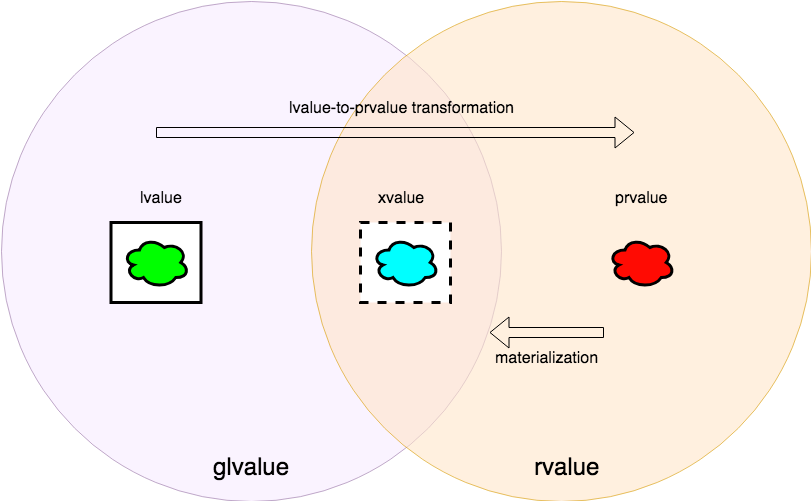
\includegraphics[width = \textwidth,align=c,keepaspectratio]{pictures/value_categories.png}

\end{frame}

\begin{frame}{Трансформации категорий значений}

\begin{large}lvalue -> rvalue\end{large} \\ \vspace{0.5em}
glvalue выражение может быть неявно преобразовано к prvalue. Смыслом преобразования будет копирование/использование значения исходного выражения.
\vspace{1em}

\begin{large}Временная материализация\end{large} \\ \vspace{0.5em}
prvalue может быть неявно преобразовано к xvalue. Эффектом будет инициализация временного объекта нужного типа значением-результатом исходного выражения.
\vspace{0.5em}

Примеры контекстов:
\begin{itemize}
  \setlength{\itemindent}{4em}
  \item связывание prvalue со ссылкой
  \item доступ к члену prvalue сложного типа
  \item применение оператора sizeof к prvalue
  \item контекст игнорирования результата
\end{itemize}

\end{frame}

\begin{frame}{Числовые расширения}

Значения интегральных типов могут быть преобразованы к значениям более широких интегральных типов. Значение при этом не меняется.

Например, арифметические операции требуют типов не уже \lstinline{int}.

Возможные интегральные расширения:

\begin{itemize}
  \item \lstinline{char} / \lstinline{short} \rarr \lstinline{int}
  \item \lstinline{unsigned char} / \lstinline{unsigned short} \rarr \lstinline{int} (если размер \lstinline{int} на данной платформе позволяет), либо \lstinline{unsigned}
  \item \lstinline{char} \rarr \lstinline{int} (если на данной платформе он \lstinline{signed}), либо \lstinline{unsigned}
  \item \lstinline{bool} \rarr \lstinline{int} (\lstinline{false} \rarr \lstinline{0}, \lstinline{true} \rarr \lstinline{1})
\end{itemize}

\vspace{0.5em}
Значение \lstinline{float} может быть преобразовано к значению \lstinline{double}.

\end{frame}

\begin{frame}{Интегральные преобразования}

Могут менять значение.
\vspace{1.5em}

Значение одного интегрального типа может быть преобразовано к значению другого интегрального типа:

\vspace{1em}
\begin{itemize}
  \item если результат беззнаковый, то результирующее значение -- результат деления по модулю на $2^n$ \vspace{0.5em}
  \item если результат знаковый, то, если значение представимо в результирующем типе -- оно не меняется, если нет -- то результат зависит от реализации \vspace{0.5em}
  \item если исходный тип -- \lstinline{bool}, то \lstinline{false} \rarr \lstinline{0}, \lstinline{true} \rarr \lstinline{1}
\end{itemize}

\end{frame}

\begin {frame}{Преобразования с плавающей точкой}

Значение одного FP типа может быть преобразовано к значению другого FP типа:

\begin{itemize}
  \item если исходное значение представимо, оно не меняется
  \item если исходного значение находится между двух представимых значений результирующего типа -- оно приводится к одному из них
  \item иначе -- UB
\end{itemize}
\vspace{0.5em}

Значение FP может быть преобразовано к целочисленному путём отбрасывания дробной части. Если целая часть не представима в результирующем типе, то это UB.
\vspace{1em}

Целочисленное значение может быть преобразовано к FP, возможно неточно.

\end{frame}

\begin{frame}{Преобразования к \lstinline{bool}}

Значение целочисленного типа, FP, \lstinline{enum}, указателя может быть преобразовано к значению \lstinline{bool}.
\vspace{1em}

\begin{itemize}
  \item нулевое исходное значение (в т.ч. нулевой указатель) преобразуется к \lstinline{false} \vspace{1em}
  \item любое другое исходное значение преобразуется к \lstinline{true}
\end{itemize}

\end{frame}

\begin{frame}{Стандартные арифметические преобразования}

Стандартные арифметические операции требуют операндов одного типа. К операндам разных арифметических типов применяются неявные преобразования (после числовых расширений):
\vspace{1em}

\begin{itemize}
  \item если один из операндов имеет тип \lstinline{long double}, то другой также преобразуется к \lstinline{long double} \vspace{0.5em}
  \item если один из операндов имеет тип \lstinline{double}, другой также преобразуется к \lstinline{double} \vspace{0.5em}
  \item если один из операндов имеет тип \lstinline{float}, другой также преобразуется к \lstinline{float} \vspace{0.5em}
\end{itemize}

\end{frame}

\begin{frame}{Стандартные арифметические преобразования, продолжение}

\begin{itemize}
  \item если оба операнда знаковые или беззнаковые, то операнд меньшего ранга преобразуется к рангу другого операнда \vspace{0.5em}
  \item если ранг беззнакового операнда больше или равен рангу знакового, знаковый преобразуется к беззнаковому \vspace{0.5em}
  \item если тип знакового операнда может представить все значения типа беззнакового операнда, беззнаковый операнд преобразуется к типу знакового \vspace{0.5em}
  \item оба операнда преобразуются к беззнаковому варианту типа знакового операнда
\end{itemize}
\vspace{0.5em}

Ранг: \lstinline{bool < signed char < short < int < long < long long}.

\end{frame}

%-------------------------------------------------

\section{Объекты}

\begin{frame}{Объекты}

Это некоторая хранимая сущность, представляющая собой данные, которыми оперирует программа.

Характеризуется:
\begin{itemize}
  \item размером (\lstinline[basicstyle=\ttfamily\small]{sizeof} для определения размера)
  \item выравниванием (\lstinline[basicstyle=\ttfamily\small]{alignof} для определения выравнивания)
  \item типом размещения (автоматический, статический, динамический, тред-локальный)
  \item временем жизни
  \item типом
  \item значением (возможно, неопределенным)
  \item именем (не обязательно)
\end{itemize}

Что \emph{не} является объектом (примеры): значение, ссылка, функция, не статический член класса, \lstinline[basicstyle=\ttfamily\small]{this}.

\end{frame}

\begin{frame}{Объекты}

Для любого объекта типа T можно говорить
\begin{itemize}
  \item об объектном представлении: последовательность байт, количеством равным размеру T, начинающаяся по тому же адресу, что и размещение объекта
  \item о представлении значения: последовательность бит, формирующая значение объекта
\end{itemize}

Объектное представление не обязательно эквивалентно представлению значения: например, из-за padding. \vspace{0.5em}

Подобъекты: члены классов, представления базовых классов, элементы массивов. \vspace{0.5em}

Размер любого полного объекта должен быть не меньше 1. \vspace{0.5em}

Любые два объекта, времена жизни которых пересекаются, должны иметь разные адреса.

\end{frame}

\begin{frame}{cv-квалификаторы}

Тип может иметь т.н. cv-квалификатор: \lstinline[basicstyle=\ttfamily\small]{const}, \lstinline[basicstyle=\ttfamily\small]{volatile} или \lstinline[basicstyle=\ttfamily\small]{const volatile}.

Это является частью типа соответствующего объекта (переменной). \vspace{1em}

\begin{itemize}
  \item \lstinline[basicstyle=\ttfamily\small]{const}: после инициализации, значение объекта не может меняться \vspace{1em}
  \item \lstinline[basicstyle=\ttfamily\small]{volatile}: любой доступ к такому объекту должен быть частью наблюдаемого поведение программы
\end{itemize}

\vspace{1em}

Допустимо неявное преобразование от менее строгого варианта к более строгому.

\end{frame}

\begin{frame}{Переменные}

Переменной называют объект или ссылку (не являющуюся нестатическим членом класса), ассоциированные с идентификатором посредством объявления. \vspace{1em}

У любой переменной есть область видимости, которая начинается с момента объявления и заканчивается концом блока или пространства имен, в котором она была объявлена. \vspace{1.5em}

Локальная переменная: переменная, объявленная в блоке или аргумент функции. \vspace{1em}

Глобальная переменная: переменная, объявленная на уровне пространства имен. \vspace{1em}

\end{frame}

\begin{frame}{Типы размещения}

\begin{itemize}

  \item автоматический: объект автоматически размещается в начале блока, в котором он объявлен, и удаляется при выходе из этого блока \vspace{1em}
  
  \item статический: объект размещается в начале работы программы и удаляется в конце; образ программы содержит только один экземпляр этого объекта \vspace{1em}
  
  \item тред-локальный: объект размещается при создании треда и удаляется при удалении треда; каждый тред в программе имеет свой экземпляр этого объекта \vspace{1em}
  
  \item динамический: размещением и удалением управляет программа

\end{itemize}

\end{frame}

\begin{frame}{Назначение типов размещения}

По умолчанию:
\begin{itemize}
  \item локальные переменные имеют автоматический тип размещения \vspace{0.5em}
  \item глобальные переменные имеют статический тип размещения
\end{itemize}

\vspace{2em}

Явное назначение:
\begin{itemize}
  \item спецификатор \lstinline{static} в объявлении локальной переменной -- статический тип размещения \vspace{0.5em}
  \item спецификатор \lstinline{thread_local} в объявлении переменной -- тред-локальный тип размещения
\end{itemize}

\end{frame}

\begin{frame}[fragile]{Примеры размещений}
\begin{lstlisting}[basicstyle=\ttfamily\small]

int static_global = 10; // global static

unsigned next_int()
{
    static unsigned state = 0; // local static
    return state++;
}

void thread_body()
{
    thread_local unsigned thread_state = next_int(); // thread local
    char c = '\n'; // local automatic
}

\end{lstlisting}
\end{frame}

\begin{frame}{Временные объекты}

Материализация: временный объект создается из prvalue, когда контекст требует glvalue. \vspace{1.5em}

Временные объекты удаляются в конце исполнения полного выражения (в т.ч. в случае прерывания исполнения исключением). \vspace{1.5em}

Если внутри выражения было создано более одного временного объекта, то они удаляются в порядке, обратным порядку их создания. \vspace{1.5em}

Время жизни временного объекта может быть продлено константной lvalue ссылкой или rvalue ссылкой. \vspace{1.5em}

\end{frame}

\end{document}
